\chapter{Probabilistic Models}

A structured probabilistic model is a probabilistic model for which a graph is used to describe the conditional dependence structure between random variables. Basically, they provide a formalism for representing complex probability distributions in a way that captures the dependencies and independencies between random variables. 

Having the following random variables $ x_1, x_2, x_3, x_4 $ with its independent associated probability $ P ( x_1), P(x_2), P(x_3), P(x_4) $ there are different ways to represent the joint probability $ P \left( x_1, x_2, x_3, x_4  \right)  $ that represent the interactions in a probability distribution using a graph. Graphical models can be largely divided into two categories: models based on directed acyclic graphs, and models based on undirected graphs. 


\begin{figure}[h]
    \centering
    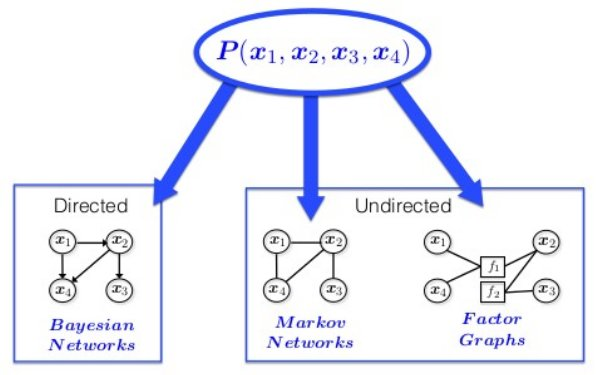
\includegraphics[width=8cm]{Images/structured-probabilistic.jpg}
    \caption{Directed and undirected networks}
\end{figure}

\section{Directed Models}

One kind of structured probabilistic model is the directed graphical model, otherwise known as the belief network or Bayesian network. Directed models are applicable to situations where the causality only flows in one direction. The direction of the arrow indicates which variable’s probability distribution is defined in terms of the other’s.

\begin{figure}[h]
    \centering
    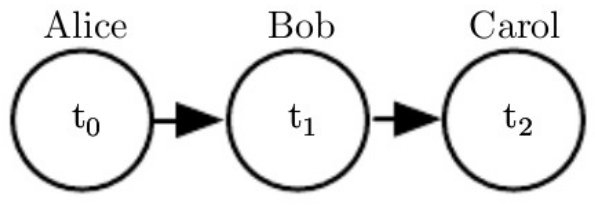
\includegraphics[width=6cm]{Images/directed-network.jpg}
    \caption{Directed networks}
    \label{fig:directed-networks}
\end{figure}

\newpage

\noindent Depending on the degrees of dependence between the different variables we will build different Bayesian networks and the joint probability factorization will also be different.

\begin{figure}[h]
    \centering
    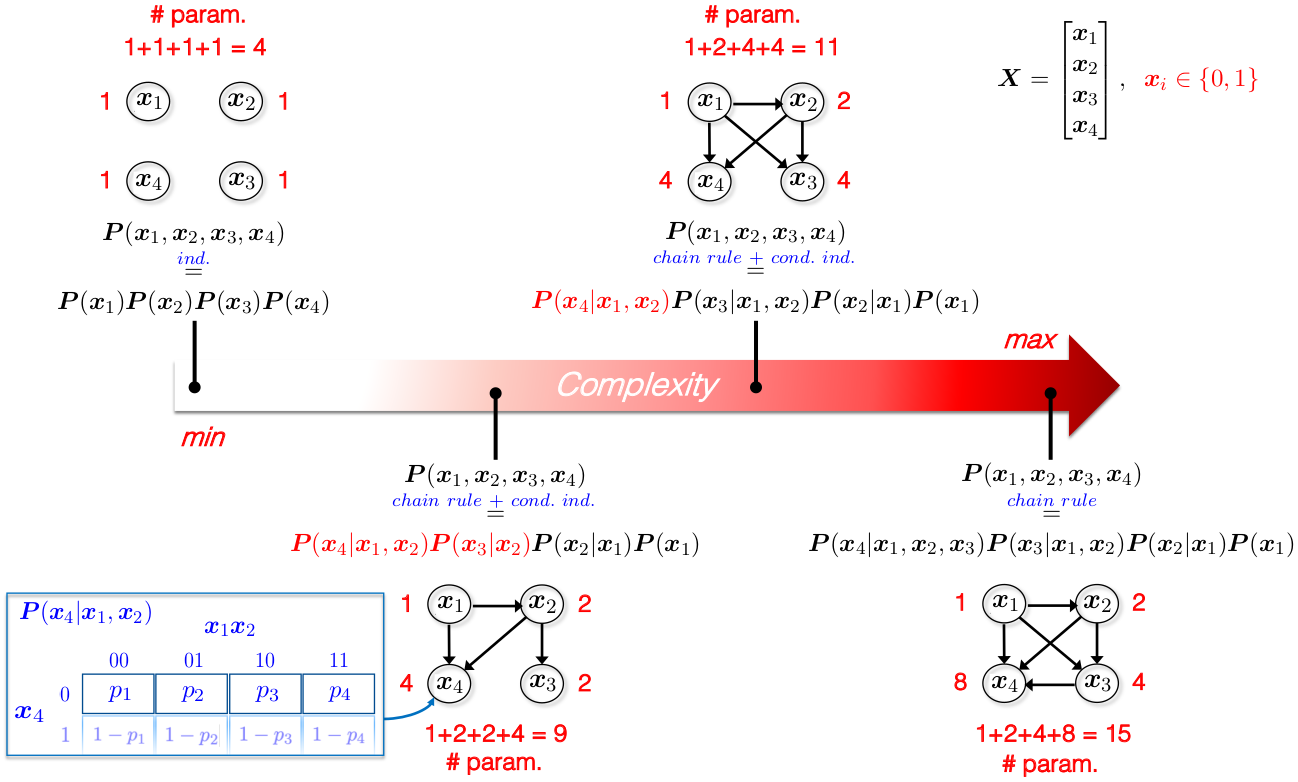
\includegraphics[width=15cm]{Images/joint-probability.png}
    \caption{Joint probability}
    \label{fig:joint-probability}
\end{figure}

\noindent Where the joint probability factorization is found by applying the product rule and using conditional independence to simplify factors. In general we can say:

$$ P(x_1, ..., x_n) = \prod_{i=1}^n P(x_i | pa_G (x_i)) $$

where $pa_G(x_i)$ is the parent nodes of $x_i$.

\noindent Since the variables $x_1, x_2, x_3, x_4$ are binary the number of parameters needed to define it will vary with the number of parents. Therefore, for the case of having an independent variable $x_i$ we will have 1 parameter, if we have a variable with one parent node we will have 2 parameters, with 2 parent nodes 4 parameters, with 3 parent nodes 8 parameters, etc. 



\section{Undirected Models}

Undirected models are used when influence has no clear direction or the influence flows in both directions.

\begin{figure}[h]
    \centering
    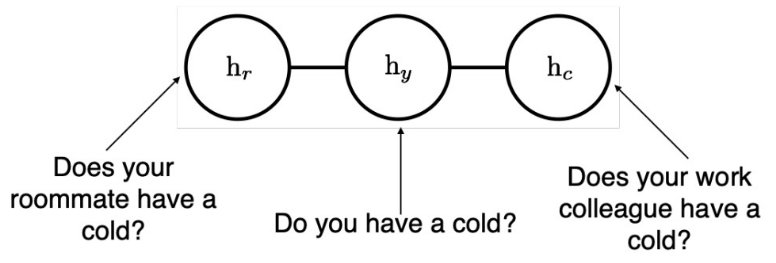
\includegraphics[width=8cm]{Images/undirected-network.jpg}
    \caption{Undirected networks}
    \label{fig:undirected-networks}
\end{figure}

\newpage

\noindent Formally, an undirected graphical model is a structured probabilistic model defined on an undirected graph $G$. For each clique $C$ in the graph, a factor $\phi(C)$ measures the affinity of the variables in that clique for being in each of their possible joint states. Together they define an unnormalized probability distribution.

$$ \tilde{p}(x) = \prod_{C \in G} \phi(C)  $$


\noindent A clique of the graph is a subset of nodes that are all connected to each other by an edge of the graph.

\begin{figure}[h]
    \centering
    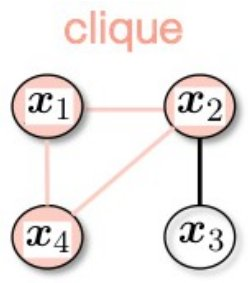
\includegraphics[width=3cm]{Images/clique.jpg}
    \caption{Clique of a undirected network}
    \label{fig:clique}
\end{figure}

\noindent To obtain a valid probability distribution, we must use the corresponding normalized probability distribution:

$$ p(x) = \frac{1}{Z} \tilde{p} (x)$$

where $Z$ is the value that results in the probability distribution summing or integrating to 1:

$$ Z = \int{ \tilde{p}(x) dx }$$

\noindent The normalizing constant $Z$ is known as the partition function. Since $Z$ is an integral or sum over all possible joint assignments of the state $x$ it is often intractable to compute.

\subsection{Energy Based Models}

Many interesting theoretical results about undirected models depend on the assumption that $\forall ~ x $, $\hat{p} (x) > 0$. A convenient way to enforce this condition is to use an energy-based model. We can enforce $\phi(C) > 0$ by defining the unnormalized probability distribution as: 

$$ \hat{p}(x) = \exp{(-E(x))} $$

where $E(x)$ is known as the energy function. 

\noindent Different cliques will also correspond to different terms of the energy function.

$$ \exp{(-E(x))} = \exp{\left(-\sum_{C \in G} E_C(x_C)\right)} $$

where $E_C$ and $x_C$ are the energy term and the subset of variables associated to clique $C$, respectively.

\noindent Any distribution of the form is an example of a Boltzmann distribution. For this reason, many energy-based models are called Boltzmann machines.


\section{Separation}

In structured probabilistic models, separation refers to a concept that helps identify conditional independence relationships between random variables given the observed variables in the model. In undirected graphs separation is related to the Markov properties that dictate the conditional independence relationships in the graph.

\begin{itemize}
    \item Nodes are conditionally independent of their non-neighbors given their neighbors.
    \item Non-adjacent nodes are conditionally independent given the set of nodes separating them.
    \item The entire set of nodes is conditionally independent of any subset of nodes that separates it
\end{itemize}

\begin{figure}[h]
    \centering
    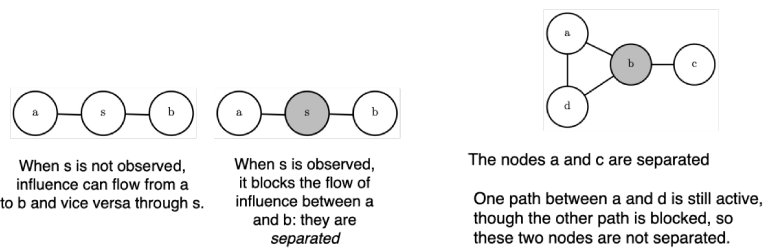
\includegraphics[width=13cm]{Images/separation.png}
    \caption{Separation in undirected graphs}
\end{figure}


\subsection{D-Separation}

In the case of directed graphs, we need to consider d-separation, or directed separation which is the criterion used in Bayesian networks to determine whether two sets of nodes are conditionally independent given a third set. The concept is based on the idea of blocking paths of influence between variables. The rules for d-separation are the following:

\begin{itemize}
    \item Active Trail. A trail between two variables is considered active if it is not blocked. Active trails allow the flow of influence between variables. 
    \item Blocking. A trail can be blocked by the presence of certain variables. There are three types of variables able to block a trail: If a variable is observed (given), it blocks the trail, if a collider (a node with two incoming edges) is not observed or one of its descendants is observed, it blocks the trail and if a non-collider is not observed, it blocks the trail.

\end{itemize}

\begin{figure}[h]
    \centering
    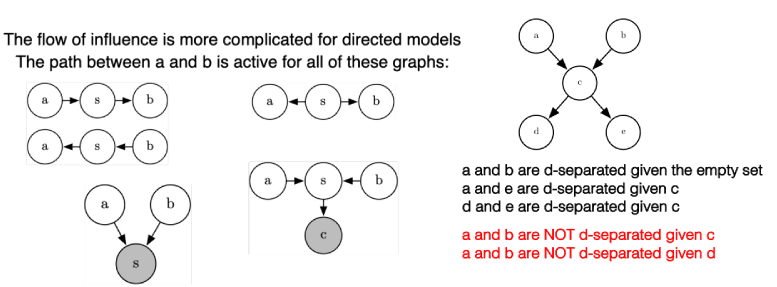
\includegraphics[width=15cm]{Images/d-separation.png}
    \caption{D-Separation in directed graphs}
\end{figure}


\newpage
\section{Sampling}

Graphical models play a crucial role in simplifying the process of generating samples from a given model. Directed models, for instance, offer a convenient method for swiftly obtaining unbiased samples that represent the entire model. To achieve this, they employ a technique known as ancestral sampling. This method involves sequentially sampling nodes in a topological order based on the influence of their parent nodes. However, challenges arise when trying to sample specific nodes that are conditioned on observed nodes that don't initiate the topological order. In spite of these challenges, directed models still provide an efficient and straightforward means of sampling through ancestral sampling.

\noindent In contrast, when dealing with undirected models, the process of generating samples employs Gibbs sampling, an iterative technique. Unlike in the case of directed models, exact sampling cannot be achieved in undirected models due to the lack of a simple closed-form expression. Instead, multiple iterations are necessary to progressively approximate the joint distribution with greater accuracy. Gibbs sampling operates by sampling individual variables one at a time while conditioning them on the rest, gradually approaching convergence with the true distribution. The number of iterations required depends on the complexity of the model and the desired level of accuracy.